\subsection{Standaard Taylorreeksen}\label{subsec:standaardTaylorreeksen}
Onthoud: de cosinus is even (symmetrisch rond de $y$-as) en deze heeft even machten, evenzo is de sinus oneven.
De standaard Taylorreeksen rond 0 om te onthouden zijn
\begin{align*}
    \cos x &\coloneqq \sum_{n=0}^\infty (-1)^n \frac{x^{2n}}{(2n)!} \\
    \sin x &\coloneqq \sum_{n=0}^\infty (-1)^n \frac{x^{2n+1}}{(2n+1)!} \\
    e^x &\coloneqq \sum_{n=0}^\infty \frac{x^n}{n!} \\
    \ln (1+x) &= \sum_{n=0}^\infty (-1)^{n} \frac{x^{n+1}}{n+1} \\
    \arctan x &= \sum_{n=0}^\infty (-1)^n \frac{x^{2n+1}}{2n+1} \\
\end{align*}
De reeks van $\sqrt{1+x}$ kun je vinden door te stellen
\begin{align*}
    \left( c_0 + c_1 x + c_2 x^2 + \dotsm \right)^2 &= 1+x \\
    c_0^2 + 2 c_0 c_1 x + \dotsm &= 1+x
\end{align*}
waaruit de eerste paar termen snel te vinden zijn, namelijk $c_0=1$ en dus $c_1 = \frac 1 2$ enzovoorts.

Merk op dat inderdaad
\[
    \ln \left(1 + \frac a n \right)^n = n \ln \left(1 + \frac a n \right) = n \left(\frac a n - \frac{a^2}{2n^2} + \dots \right) \upto{n \to \infty} a.
\]
\subsection{Gonioformules} \label{gonioformules}
\subsubsection{Waardes van de sinus en de cosinus}
\begin{figure}[h!]
    \centering
    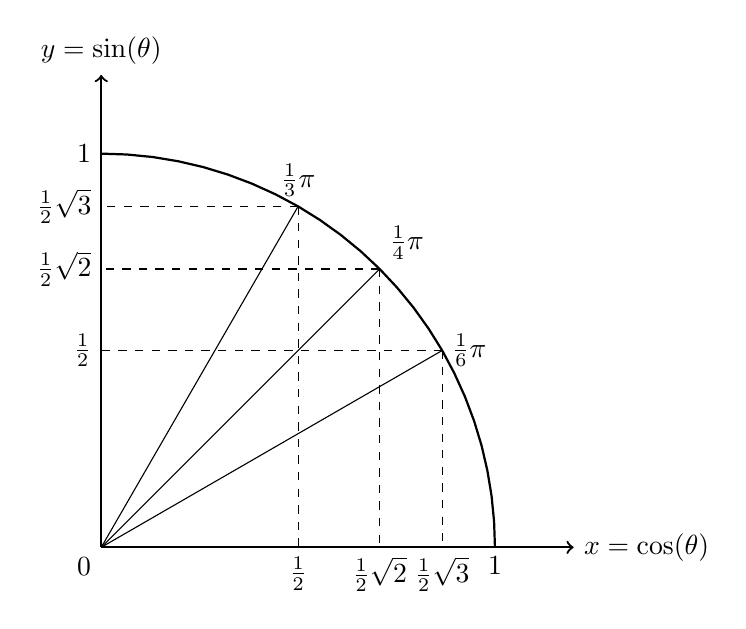
\begin{tikzpicture}[scale=5]
        \draw (1,0) node [below] {1};
        % assen
        \draw [->, thick] (0,0) -- (1.2,0) node [right] {$x = \cos(\theta)$};
        \draw [->, thick] node [below left] {0} (0,0) -- (0,1.2) node [above] {$y = \sin (\theta)$};
        % kwart cirkel
        \draw [thick,domain=0:90] plot ({cos(\x)}, {sin(\x)}) node [left] {1};
        % driehoeken
        \draw (0,0) -- (.866, .5) node [right] {$\frac{1}{6} \pi$};
        \draw [dashed] (.866, .5) -- (.866, 0) node [below] {$\frac{1}{2} \sqrt{3}$};
        \draw [dashed] (.866, .5) -- (0, .5) node [left] {$\frac{1}{2}$};
        \draw (0,0) -- (.707, .707) node [above right] {$\frac{1}{4} \pi$};
        \draw [dashed] (.707, .707) -- (.707, 0) node [below] {$\frac{1}{2} \sqrt{2}$};
        \draw [dashed] (.707, .707) -- (0, .707) node [left] {$\frac{1}{2} \sqrt{2}$};
        \draw (0,0) -- (.5, .866) node [above] {$\frac{1}{3} \pi$};
        \draw [dashed] (.5, .866) -- (.5, 0) node [below] {$\frac{1}{2}$};
        \draw [dashed] (.5, .866) -- (0, .866) node [left] {$\frac{1}{2} \sqrt{3}$};
    \end{tikzpicture}
\end{figure}

\subsubsection{Verdubbelingsformules}

De verdubbelingsformules kunnen we afleiden met behulp van e-machten.
We gebruiken
\begin{align*}
    \cos x = \frac 1 2 \left( e^{ix} + e^{-ix} \right) \\
    \sin x = \frac 1 {2i} \left( e^{ix} - e^{-ix} \right) \\
\end{align*}
en als je niet meer weet waar de plussen en de minnen zaten dan vul je $\cos 0 = 1$ of $\sin 0 = 0$ in.

Nu schrijven we
\begin{align*}
    2 \cos x \sin x &= 2 \cdot \frac 1 2 \left( e^{i x} + e^{-ix} \right) \frac 1 {2i} \left( e^{ix} - e^{-ix} \right) \\
    &= \frac 1 {2i} \left(e^{2 i x} - e^{-2ix} \right) \\
    &= \sin 2 x
\end{align*}
en evenzo
\begin{align*}
    \cos^2 x - \sin^2 x &= \frac 1 4 \left( e^{ix} + e^{-ix} \right)^2 - \frac 1 {2i} \frac 1 {2i} \left( e^{ix} - e^{-ix} \right)^2 \\
    &= \frac 1 4 \left( e^{2ix} + 2 + e^{-2ix} \right) - \frac {-1} {4} \left( e^{2ix} - 2 + e^{-2ix} \right) \\
    &= \frac {1} {2} \left( e^{2ix} + e^{-2ix} \right) \\
    &= \cos 2x \,.
\end{align*}
en dus weten we nu dat
\begin{align}
    \label{verdubbeling1}
    \cos (2\alpha) &= \cos^2 \alpha - \sin^2 \alpha  \\
    \sin (2\alpha) &= 2 \cos \alpha \sin \alpha. \label{verdubbeling2}
\end{align}


Verder is
\begin{align*}
    \cos (2 \alpha) &= \cos^2 \alpha - \sin^2 \alpha \\
    &= \cos^2 \alpha - (1 - \cos^2 \alpha ) \\
    &= 2  \cos^2 \alpha - 1
\end{align*}
en uit dezelfde regel volgt ook
\begin{align*}
    \cos (2 \alpha) &= \cos^2 \alpha - \sin^2 \alpha \\
    &= (1 - \sin^2 \alpha) - \sin^2 \alpha \\
    &= 1 - 2 \sin^2 \alpha .
\end{align*}

\subsubsection{Alternatieve afleiding voor~\eqref{verdubbeling1}}

Het idee is om $e^{i(\phi + \theta)}$ uit te schrijven en aan beide kanten het re\"eele deel te nemen.

\begin{align*}
    \cos(\phi + \theta) + i \sin(\phi + \theta) &= e^{i(\phi + \theta)} \\
    &= e^{i\phi} e^{i \theta} \\
    &= (\cos \phi + i \sin \phi )(\cos \theta + i \sin \theta) \\
    &= \cos \phi \cos \theta + i \cos \phi \sin \theta + i \sin \phi \cos \theta - \sin \phi \sin \theta \\
\end{align*}

en dus is
\begin{align*}
    \cos (\phi + \theta) &= \cos \phi \cos \theta - \sin \phi \sin \theta \\
    \implies \cos (2 \phi) &= \cos^2 \phi - \sin^2 \phi
\end{align*}

\subsection{Andere gonioformules}

Onthoud
\begin{align*}
    \sin(\alpha + \beta) &= \sin \alpha \cos \beta + \cos \alpha \sin \beta \\
    \cos(\alpha + \beta) &= \cos \alpha \cos \beta - \sin \alpha \sin \beta .
\end{align*}
Voor de formules voor $\sin(\alpha - \beta)$ en $\cos(\alpha - \beta)$, vul $-\beta$ in voor $\beta$ en gebruik dat $\cos (-\alpha) = \cos \alpha $ en $\sin (-\alpha) = - \sin \alpha $.

Merk op dat voor $\alpha = \beta$ hier de formules uit (\ref{verdubbeling1}) en (\ref{verdubbeling2}) staan.



\subsection{Cosinus en sinus hyperbolicus}\label{subsec:cosinusEnSinusHyperbolicus}

Merk op dat deze definities gelijk zijn aan de gewone sinus en cosinus maar dan niet alternerend.
\begin{align*}
    \cosh z &\coloneqq \frac{1}{2} (e^z + e^{-z}) = \sum_{k=0}^\infty \frac{z^{2k}}{(2k)!} = \text{ alle even termen van de e-machtreeks} \\
    \sinh z &\coloneqq \frac{1}{2} (e^z - e^{-z}) = \sum_{k=0}^\infty \frac{z^{2k+1}}{(2k+1)!} = \text{ alle oneven termen van de e-machtreeks}
\end{align*}

\subsection{Versimplificeren van de sinus van de arccosinus en dergelijke}\label{subsec:versimplificerenVanDeSinusVanDeArccosinusEnDergelijke}

In het geval van $\sin (\arccos \alpha)$, noem $\arccos \alpha \eqqcolon \beta$ en denk aan de driehoek met schuine zijde van lengte 1.
Nu zien we dat, omdat $\alpha = \cos \beta$, er geldt dat de lengte van de aanliggende zijde gelijk is aan $\alpha$ en dus is de overstaande zijde van lengte $\sqrt{1-\alpha^2}$.

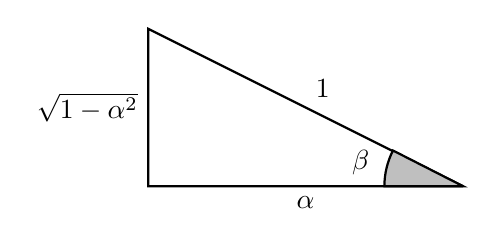
\begin{tikzpicture}[thick]
    \draw(4,0)
    -- (0,0) node[midway,below]{$\alpha$}
    -- (0,2) node[midway,left]{$\sqrt{1-\alpha^2}$} % node of point
    -- (4,0) node[midway,above right]{$1$};
    \draw[fill=lightgray, thick] (4,0)
    -- (3,0) arc (180:153:1cm) node at (2.7,0.3) {$\beta$}
    -- cycle;
\end{tikzpicture}

Nu is
\[ \sin (\arccos \alpha) = \sin \beta = \sqrt{1-\alpha^2}\,. \]
\subsection{Matrix in e-macht}\label{subsec:matrixInE-macht}
Deze definitie lijkt op de gewone definitie van $e^x$.
Als $A$ een matrix, dan geldt
\[ e^{At} \coloneqq \sum_{k=0}^\infty \frac{A^k t^k}{k!} \]
Voor $\displaystyle A = \matrix{0 & 1 \\ 1 & 0}$ geldt dan
\[ e^{At} =
\matrix{1 + \frac{t^2}{2!} + \frac{t^4}{4!} + \dots & t + \frac{t^3}{3!} + \dots \\
    t + \frac{t^3}{3!} + \dots & 1 + \frac{t^2}{2!} + \frac{t^4}{4!} + \dots}
= \matrix{\cosh t & \sinh t \\ \sinh t & \cosh t}\]
\subsection{Imaginaire e-macht}\label{subsec:imaginaireE-macht}
\begin{align*}
    e^{ix} &= \cos x + i \sin x \\
    e^{-ix} &= \sin x + i \cos x
\end{align*}